\section{Classifieur 2 : Densités et K plus proches voisins}
Liste des fonctions mentionnées dans cette section : \textit{getdensity}, \textit{computepdensities}, \textit{learningclassifier2}, \textit{decisionclassifier2}

\subsection{Principe et implémentation}

Pour compléter les données obtenues, on utilise donc une seconde méthode de classification. L'identification du chiffre est à présent réalisée à partir de la répartition des pixels noirs au sein de zones décomposant le rectangle de base. La première étape consiste donc à diviser en $m\times n$ zones le rectangle encadrant le chiffre à identifier. Il suffit ensuite de calculer la densité de pixels noirs dans chacune de ces zones.\\

Comme précédemment, le classifieur nécessite de passer par une phase d'apprentissage afin d'obtenir une base de densités de référence. Il est ensuite possible d'identifier le chiffre en comparant les densités obtenues avec les densités de référence. Les probabilités d'appartenance du chiffre à chacune des classes est finalement calculée en fonction du nombre de représentants de chaque classe parmis ses k plus proches voisins.

\subsubsection{Fonctions utilisées}

\textit{getdensity( rectangle, m, n ) : density}\\
\begin{itemize}
	\item[\textbf{Entrées :}] \textbf{base}, coordonnées du rectangle contenant le chiffre à lire, obtenues grâce au pré-traitement. \\\textbf{m}, nombre de zones qui découpent le rectange sur la hauteur. \\\textbf{n}, nombre de zones qui découpent le rectangle sur la largeur.
	\item[\textbf{Sortie :}] \textbf{density}, vecteur contenant les densités normalisées relatives à chaque zone, de dimension $mn$
\end{itemize}
Calcule la densité de pixels noirs dans chaque zone de l'image. Les zones sont obtenues par division du rectangle contenant le chiffre en m parties sur la hauteur et n parties sur la largeur. Les densités sont calculées de la manière suivante :

$$density_ij = \frac{nb pixels noirs_ij}{hauteur rectangle \times largeur rectangle}$$\\

\textit{computepdensities( vectordensity, vectordensitylearning, nbrectangleslearning, k ) : pbelonging}\\
\begin{itemize}
	\item[\textbf{Entrées :}] \textbf{vectordensity}, vecteur de densité d'un objet à identifier.\\\textbf{vectordensitylearning}, résultat de la phase d'apprentissage. \\\textbf{nbrectangleslearning}, nombre d'objets contenus dans la base d'apprentissage.\\\textbf{k}, paramètre k.
	\item[\textbf{Sortie :}] \textbf{pbelonging}, vecteur de probabilités d'appartenances de dimension 10, soit le nombre de classes d'appartenance.
\end{itemize}
Calcule la différence entre le vecteur de densités de l'objet à identifier et les vecteur de densités de chaque élément contenu dans la base d'apprentissage respectivement. On obtient un vecteur de distances de dimension \textit{taille de la base d'apprentissage}. On se place ensuite dans un espace 1d abstrait où apparaît l'objet à identifier : chaque élément de la base d'apprentissage est disposé dans cet espace en fonction de sa distance à l'objet calculée précédemment.
On sélectionne enfin les k plus proches voisins de l'objet à identifier et détermine les probabilités d'appartenance de la manière suivante :
$$pbelonging1(\omega_i/x) = \frac{k_i}{k}$$
avec $x$ l'objet testé pour la classe d'appartenance $\omega_i$ et $k_i$ le nombre de voisins appartenant à $\omega_i$ parmi les k plus proches

\subsubsection{Phase d'apprentissage}

\textit{learningclassifier2( rectangleslearning, learningimage, m, n) : vectordensitylearning}
\\
\begin{itemize}
	\item[\textbf{Entrées :}] \textbf{rectangleslearning}, coordonnées des rectangles contenant chacun des chiffres connus de la base d'apprentissage. \\\textbf{learningimage}, image d'apprentissage. \\\textbf{m, n}, nombre de zones à découper dans un rectangle respectivement en hauteur en en largeur.
	\item[\textbf{Sortie :}] \textbf{vectordensitylearning}, matrice regroupant les vecteurs de densités propres à chaque objet de la base d'apprentissage, de dimension $taille base apprentissage \times mn$
\end{itemize}

La phase d'apprentissage a pour objectif de calculer les vecteurs de densités de tous les objets de la base d'apprentissage afin de constituer une base de référence pour identifier les éléments à traiter. On obtient en sortie les vecteurs de densités de l'ensemble des composants de la base d'aprentissage qui sera utilisé lors de la phase de décision.

\subsubsection{Phase de décision}

\textit{decisionclassifier2( rectangles, image, vectordensitylearning, m, n, k) : pbelonging}
\\
\begin{itemize}
	\item[\textbf{Entrées :}] \textbf{rectangles}, coordonnées des rectangles contenant chacun des chiffres à identifier. \\\textbf{image} image à traiter. \\\textbf{m, n}, nombre de zones à découper dans un rectangle respectivement en hauteur en en largeur.
	\item[\textbf{Sortie :}] \textbf{pbelonging}, matrice de probabilités d'appartenance aux dix classes pour chaque objet à identifier, de dimension $s \times 10$, avec $s$ le nombre d'objets à identifier et $10$ le nombre de classes d'appartenance.
\end{itemize}

La phase de décision est divisée en deux étapes. D'abord, le calcul de densités est effectué sur chacun des objets à identifier, à l'image de ce qui a été réalisé en phase d'apprentissage. Une fois les vecteurs de densités obtenus, les probabilités d'appartenance de chaque objet sont calculées à l'aide de la fonction \textit{computepdensities}.

\subsection{Analyse et conclusion}

\subsubsection{Résultats obtenus}

\begin{figure}[h]
	\begin{center}
		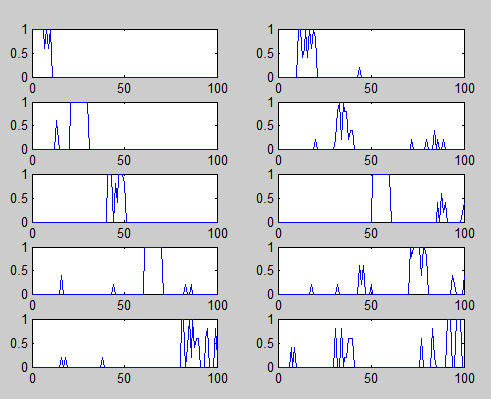
\includegraphics[width=0.8\textwidth]{img/30-pbelonging2-5555.png}
	\end{center}
	\caption{Probabilité d'appartenance à une classe pour chaque objet}
	\label{fig:proba2}
\end{figure}

On observe ici les probabilités d'appartenance de chacune des dix classes en fonction des objets x traités. Les paramètres utilisés sont les suivants : $k=5$, $m=5$ et $n=5$.
On se rapproche ici d'une fonction binaire de probabilité 1 pour les objets appartenant à la classe et 0 pour les autres, en particulier pour les classes 0, 2, 5, et 6 où les taux de reconnaissance sont particulièrement bons. On remarque également des confusions entre paires de classes : ah ouais lesquelles?

\subsubsection{Influence du paramètre $k$}

L'influence de la valeur de $k$ sur le taux de reconnaissance du classifieur 2 est très important. Comme le montre la figure ci-dessous, le meilleur taux de reconnaissance est atteint pour $k=1$ et régresse rapidement quand $k$ augmente. Ce résultat paraît surprenant : $k$ définit le nombre de voisins à considérer pour le calcul de probabilité d'appartenance et on pourrait penser que considérer un nombre relativement important de voisins aurait un effet "stabilisant" sur le taux de reconnaissance. La taille réduite de la base d'apprentissage explique peut-être ce comportement.\\
On retient donc un taux maximal pour $k=1$.

\newpage
\begin{figure}[h]
	\begin{center}
		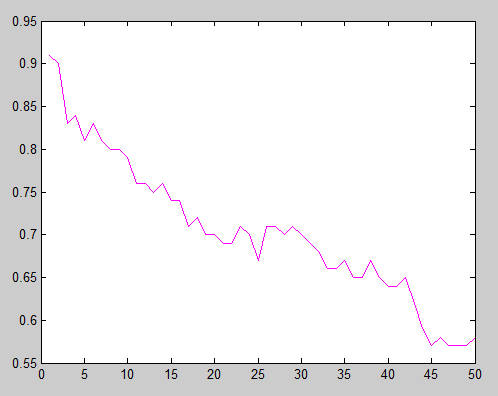
\includegraphics[width=0.5\textwidth]{img/31-influence-k.png}
	\end{center}
	\caption{Variation du taux de reconnaissance en fonction du paramètre $k$}
	\label{fig:rate2}
\end{figure}

\subsubsection{Influence des paramètres $m$ et $n$}

\begin{figure}[h]
	\begin{center}
		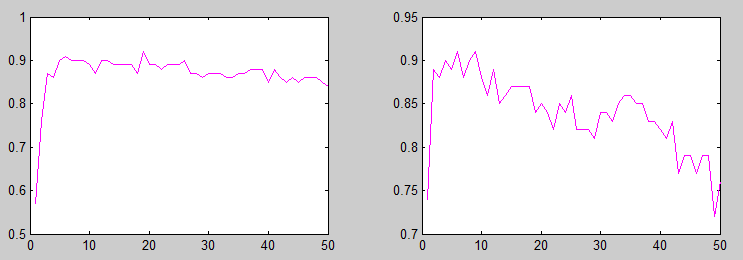
\includegraphics[width=\textwidth]{img/32-influence-m-n.png}
	\end{center}
	\caption{Variation du taux de reconnaissance en fonction des paramètres $m$ (à gauche) et $n$ (à droite)}
	\label{fig:rate1}
\end{figure}

D'après la figure ci-dessus, les influences de $m$ et de $n$ sur les résultats du classifieur 2 sont limitées. Les taux en fonction de $m$ restent en effet quasiment stable pour $5<m<50$, tandis qu'on observe une légère régression dans les taux en fonction de $n$ pour $n>5$.
On repère un taux maximal pour respectivement $m=19$ et $n=7$.

\subsubsection{Calcul des résultats avec optimisation des paramètres}

Les taux de reconnaissance du classifieur 2 montrent l'amélioration des résultats faisant suite à l'optimisation des paramètres :\\

\begin{itemize}
	\item[\textbf{$A(k=5,m=5,n=5)$ : }] $\textbf{taux de reconnaissance} = 0.83$
	\item[\textbf{$B(k=5,m=19,n=7)$ : }] $\textbf{taux de reconnaissance} = 0.83$
	\item[\textbf{$C(k=1,m=5,n=5)$ : }] $\textbf{taux de reconnaissance} = 0.90$
	\item[\textbf{$D(k=1,m=19,n=7)$ : }] $\textbf{taux de reconnaissance} = 0.90$
\end{itemize}

Résultat A : On utilise les paramètres de départs.\\
Résultat B : On optimise m et n sans changer k. Le taux de reconnaissance ne change pas.\\
Résultat C : On optimise k sans changer m et n. Le taux de reconnaissance augmente passe de 0,83 à 0,90.\\
Résultat D : On optimise k, m et n. Le taux reste inchangé à 0,90.\\
\\

Les paramètres m et n ne semblent pas influer sur le taux de reconnaissance. Pour confirmer ce résultat, on cherche à représenter à nouveau la variation du taux de reconnaissance en fonction de $m$ et $n$, avec cette fois $m$ et $n$ égaux et avec $k=1$.

\begin{figure}[h]
	\begin{center}
		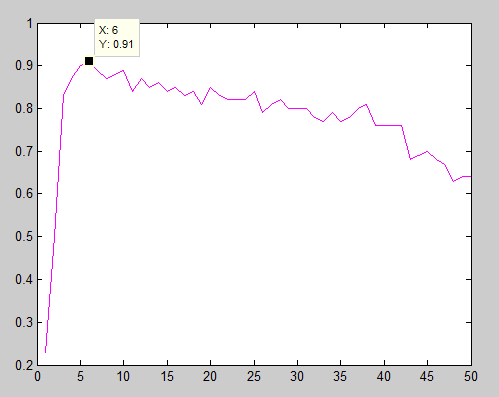
\includegraphics[width=0.8\textwidth]{img/33-influence-m=n.png}
	\end{center}
	\caption{Variation du taux de reconnaissance en fonction de $m=n$ avec $d=14$ et $k=1$ optimaux}
	\label{fig:ratemn}
\end{figure}

On obtient un nouveau maximum en $m=n=6$.

\begin{itemize}
	\item[\textbf{$E(k=1,m=6,n=6)$ : }] $\textbf{taux de reconnaissance} = 0.91$
\end{itemize}

Résultat E : On change finalement les paramètres selon ce résultat et on obtient une légère progression du taux à 0,91.